% +------------------------------------------------------------------------+
% | CGAL Reference Manual:  polyhedron.tex
% +------------------------------------------------------------------------+
% | Combinatoric and geometry of polyhedral surfaces in 
% | halfedge representation.
% |
% | 11.10.1996   Lutz Kettner
% |              Start rewriting the whole stuff
% | 
\RCSdef{\polyhedronRev}{$Revision$}
\RCSdefDate{\polyhedronDate}{$Date$}
% +------------------------------------------------------------------------+

\ccParDims

\chapter{3D-Polyhedral Surfaces}
\label{chapterPolyhedron}
\ccChapterRelease{\polyhedronRev. \ \polyhedronDate}\\
\ccChapterAuthor{Lutz Kettner}


% +------------------------------------------------------------------------+
\section{Introduction}

This chapter presents polyhedral surfaces in three dimensions. They
are a collection of vertices, edges and facets with an incidence
relationship on them. The organization beneath is a halfedge data
structure which restricts the class of representable surfaces to
orientable 2-manifolds -- with and without boundary. In the case of a
closed surface we call it a {\em polyhedron}.

\begin{ccTexOnly}
    %\vspace{-4mm}
    \begin{center}~\hspace{5cm}
      \parbox{0.55\textwidth}{%
          \includegraphics[width=0.55\textwidth]{idraw/shark.ps}%
      }
    \end{center}
    \vspace*{-16mm}
\end{ccTexOnly}

\begin{ccHtmlOnly}
    <CENTER>
        <img src="./shark.gif" alt="Shaded Rendering of a Shark Model"><P>
    </CENTER>
\end{ccHtmlOnly}

\subsection*{Design Rationale}

Chapter~\ref{chapterHds} gives a design overview of the
\ccc{Halfedge_data_structure} concept, its flexibility, predefined
models and their potential use in data structures such as polyhedral
surfaces, see also~\cite{k-ddsps-98}. A halfedge data structure is an
edge-centered data structure. Each edge is decomposed into two
halfedges with opposite orientations. Functions are provided to access
incident facets and vertices. For a facet or a vertex one of the
incident halfedges can be accessed. A halfedge data structure is
responsible of storing the halfedges, vertices and facets, as well as
maintaining their incidences through a pointer based interface.

A polyhedral surface is based on a model of the
\ccc{Halfedge_data_structure} concept and adds combinatorial integrity
(e.g. internal pointers cannot be simply written), abstract concepts
to access the items, such as iterators and circulators, high level
operations and ease-of-use, for example Euler operators. It also adds
knowledge about the geometric information kept in the data structure,
such as points or plane equations, with a traits class.

The class \ccc{Polyhedron} can store polyhedra and polyhedral
surfaces. The template argument for the \ccc{Halfedge_data_structure}
allows to choose among the different possible models, for example a
list or a vector based representation.  Using a vector provides random
access for the elements in the polyhedral surface and is more space
efficient, but elements cannot be deleted arbitrarily. Using a list
allows arbitrary deletions, but provides only bidirectional iterators
and is less space efficient. The provided default model for the
halfedge data structure
\ccc{Halfedge_data_structure_polyhedron_default_3<R>} chooses the
list representation and \ccc{Point_3<R>} for the geometric
information stored with vertices and \ccc{Plane_3<R>} for the
geometric information stored with facets.

A utility class \ccc{Polyhedron_incremental_builder_3} helps in
creating polyhedral surfaces from a list of points followed by a list
of facets represented as indices into the point list. This is
particularly useful in combination with usual file formats for polyhedra.

\subsection*{Organization of this Chapter}

Section~\ref{sectionPolyhedron} introduces the polyhedral surface
class \ccc{Polyhedron_3}, its three local classes \ccc{Vertex},
\ccc{Halfedge}, and \ccc{Facet}. Section~\ref{sectionPolyTraits}
defines the \ccc{Polyhedron_traits} concept, which adds the geometric
knowledge to the polyhedral surface, and
Section~\ref{sectionPolyTraitsModels} names the provided models for
this concept.  Section~\ref{sectionPolyHds} presents additional
requirements for the \ccc{Halfedge_data_structure} concept that were
recognized by the polyhedral surface and states the default models
that fulfills these requirements, see also Chapter~\ref{chapterHds} on
halfedge data structure. Section~\ref{sectionPolyIncrBuilder}
continues with the description of the utility class for incremental
construction of polyhedral surfaces.
Section~\ref{sectionPolyExamples} concludes this chapter with examples
using polyhedral surfaces.

% +========================================================================+
\begin{ccClassTemplate}{Polyhedron_3<Traits,HDS>}
\ccSection{Polyhedral Surfaces}
% +========================================================================+
\label{sectionPolyhedron}
\ccCreationVariable{P}

\ccDefinition  



A polyhedral surface \ccClassTemplateName\ in three dimensions
consists of vertices $V$, edges $E$, facets $F$ and an incidence
relation on them.  Each edge is represented by two halfedges with
opposite orientations.

\begin{ccTexOnly}
    \vspace{-7mm}
    \begin{center}
      \parbox{0.4\textwidth}{%
          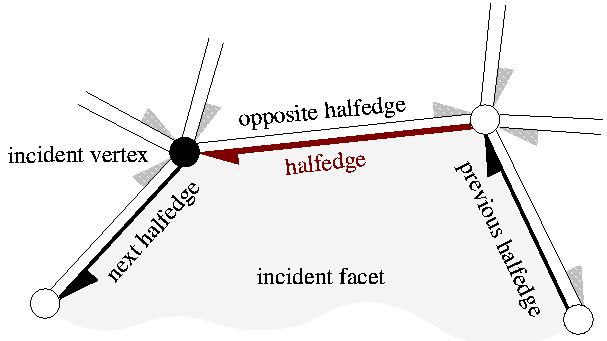
\includegraphics[width=0.4\textwidth]{idraw/halfedge.ips}%
      }
    \end{center}
    \vspace{-5mm}
\end{ccTexOnly}

\begin{ccHtmlOnly}
    <CENTER>
    <A HREF="./halfedge.gif">
        <img src="./halfedge_small.gif" alt="Halfedge Diagram"></A><P>
    </CENTER>
\end{ccHtmlOnly}

Vertices represent points in space. Edges are straight line segments
between two endpoints. Facets are planar polygons without holes
defined by the circular sequence of halfedges along their boundary.
The polyhedral surface itself is allowed to have holes. The halfedges
along the boundary of a hole are called {\em border halfedges\/} and
have no incident facets. An edge is a {\em border edge\/} if one of
its halfedges is a border halfedge.  A surface is {\em closed\/} if it
contains no border halfedges. A closed surface is a boundary
representation for polyhedra in three dimensions. The convention is
that the halfedges are oriented counterclockwise around facets as seen
from the outside of the polyhedron. An implication is that the
halfedges are oriented clockwise around the vertices. The notion of
the solid side of a facet as defined by the halfedge orientation
extends to polyhedral surfaces with border edges although they do not
define a closed object. If normal vectors are considered for the
facets, normals point outwards (following the right hand rule).

One implication of the definition is that the polyhedral surface is
always an orientable and oriented 2-manifold with border edges,
i.e.~the neighborhood of each point on the polyhedral surface is
either homeomorphic to a disc or to a half disc, except for vertices
where many holes and surfaces can meet. Another implication is that
the smallest representable surface is a triangle (for polyhedral
surfaces with border edges) or a tetrahedron (for polyhedra). Boundary
representations of orientable 2-manifolds are closed under Euler
operations. They are extended with operations that create or close
holes in the surface.

Other intersections besides the incidence relation are not allowed,
although they are not automatically handled, since self intersections
are not easy to check efficiently. \ccClassTemplateName\ does only
maintain the combinatorial integrity of the polyhedral surface (using
Euler operations) and does not consider the coordinates of the points
or any geometric information.

The class \ccClassTemplateName\ can represent polyhedral surfaces as
well as polyhedra. The interface is designed in such a way that it
is easy to ignore border edges and work only with polyhedra.

The sequence of edges can be ordered in the data structure on request
such that the sequence starts with the non-border edges and ends with
the border edges. Border edges are then itself ordered such that the
halfedge which is incident to the facet came first and the halfedge
incident to the hole came thereafter. This normalization step counts
simultaneously the number of border edges. This number is zero if and
only if the surface is a closed polyhedron. Note that this class does
not maintain this counter during further modifications. There is no
automatic caching done for auxiliary information.

The class \ccc{Polyhedron_3<Traits,HDS>} expects a model of the
\ccc{Polyhedron_traits} concept from Section~\ref{sectionPolyTraits}
as a first template argument, and a model of the
\ccc{Halfedge_data_structure} concept from Section~\ref{sectionHds}
with the additional requirements from Section~\ref{sectionPolyHds} as a second
template argument.

\ccInclude{CGAL/Polyhedron_3.h}


% +-----------------------------------+
\ccTypes

\ccTwo{Polyhedron_3<Traits>:: Halfedge_vertex_circulaM}{}

\ccNestedType{Traits}{traits class.}
\ccGlue
\ccNestedType{Halfedge_data_structure}{halfedge data structure \ccc{HDS}.}
\ccGlue
\ccNestedType{Vertex}{vertex type\lcHtml{, \ccc{Polyhedron_Vertex}}.}
\ccGlue
\ccNestedType{Halfedge}{halfedge type\lcHtml{, \ccc{Polyhedron_Halfedge}}.}
\ccGlue
\ccNestedType{Facet}{facet type\lcHtml{, \ccc{Polyhedron_Facet}}.}
\ccGlue
\ccNestedType{Size}{type for size values.}
\ccGlue
\ccNestedType{Difference}{type for difference values.}

Types for the (optionally) associated geometry. If
the specific item is not supported the type is \ccc{void*}.

\ccNestedType{Point}{point stored in vertices.}
\ccGlue
\ccNestedType{Plane}{plane equation stored in facets.}
\ccGlue
\ccNestedType{Normal}{normal vector stored in facets.}

The following handles, iterators and circulators have appropriate
non-mutable counterparts. The mutable types are assignable to their
non-mutable counterparts.  Both circulators are assignable to the
\ccc{Halfedge_iterator}. The iterators are assignable to the
respective handle types. Wherever the handles appear in function
parameter lists, the appropriate iterator can be used as well.

The iterator category is defined through the polyhedron traits class
for all iterators. The circulators are bidirectional if the halfedge
in the polyhedron traits class provides a member function
\ccc{prev()}, otherwise they are of the forward category.

\ccNestedType{Vertex_handle}{handle to vertex.}
\ccGlue
\ccNestedType{Halfedge_handle}{handle to halfedge.}
\ccGlue
\ccNestedType{Facet_handle}{handle to facet.}

\ccNestedType{Vertex_iterator}{iterator over all vertices.}
\ccGlue
\ccNestedType{Halfedge_iterator}{iterator over all halfedges.}
\ccGlue
\ccNestedType{Facet_iterator}{iterator over all facets.}

\ccNestedType{Halfedge_around_vertex_circulator}{circulator of
  halfedges around a vertex.}
\ccGlue
\ccNestedType{Halfedge_around_facet_circulator}{circulator of
  halfedges around a facet.}

\ccNestedType{iterator_category}{iterator category of all the iterators.}
\ccGlue
\ccNestedType{circulator_category}{circulator category of all the circulators.}

% +-----------------------------------+
\ccCreation

\ccThree{Halfedge_iterator}{AP.m}{}
\ccThreeToTwo

\ccConstructor{Polyhedron_3(const Traits& traits = Traits());}{}

\ccConstructor{Polyhedron_3( Size v, Size h, Size f,
                                 const Traits& traits = Traits());}
              {a polyhedron \ccVar\ with storage reserved
               for $v$ vertices, $h$ halfedges, and $f$ facets. The
               reservation sizes are a hint for optimizing storage
               allocation.}

\ccMethod{void reserve( Size v, Size h, Size f);}{reserves storage
               for $v$ vertices, $h$ halfedges, and $f$ facets. The
               reservation sizes are a hint for optimizing storage
               allocation. If the \ccc{capacity} is already greater
               than the requested size nothing happens. If the
               \ccc{capacity} changes all iterators and circulators
               might invalidate.}

\ccMethod{Halfedge_handle make_tetrahedron();}{
    adds a new tetrahedron to the polyhedral surface. 
    Returns an arbitrary halfedge of the tetrahedron.}

\ccMethod{Halfedge_handle make_tetrahedron(const Point& p1, 
                                           const Point& p2,
                                           const Point& p3, 
                                           const Point& p4);}{
    adds a new tetrahedron to the polyhedral surface with its
    vertices initialized with $p_1, p_2, p_3$ and $p_4$. Returns that
    halfedge of the tetrahedron which incident vertex is initialized
    with $p_1$, the incident vertex of the next halfedge with $p_2$,
    and the vertex thereafter with $p_3$.
    The remaining fourth vertex is initialized with $p_4$}
\vspace{-3mm}

\ccMethod{Halfedge_handle make_triangle();}{
    adds a new triangle with border edges to the polyhedral surface. 
    Returns an arbitrary, non-border halfedge of the triangle.}
\vspace{-3mm}

\ccMethod{Halfedge_handle make_triangle(const Point& p1, 
                                        const Point& p2,
                                        const Point& p3);}{
    adds a new triangle with border edges to the polyhedral surface with its
    vertices initialized with $p_1, p_2$ and $p_3$. Returns that
    non-border halfedge of the triangle which incident vertex is initialized
    with $p_1$, the incident vertex of the next halfedge with $p_2$,
    and the vertex thereafter with $p_3$.}
\vspace{-3mm}

% +-----------------------------------+
\ccHeading{Access Member Functions}
\ccThree{Halfedge_iterator}{P.size_of_border_halfedges();}{}

\ccMethod{Size size_of_vertices() const;}
    {number of vertices.}
\ccGlue
\ccMethod{Size size_of_halfedges() const;}
    {number of halfedges (incl.\ border halfedges).}
\ccGlue
\ccMethod{Size size_of_facets() const;}
    {number of facets.}

\ccMethod{Size capacity_of_vertices() const;}
    {space reserved for vertices.}
\ccGlue
\ccMethod{Size capacity_of_halfedges() const;}
    {space reserved for halfedges.}
\ccGlue
\ccMethod{Size capacity_of_facets() const;}
    {space reserved for facets.}

\ccMethod{std::size_t bytes() const;}
    {bytes used for the polyhedron.}
\ccGlue
\ccMethod{std::size_t bytes_reserved() const;}
    {bytes reserved for the polyhedron.}


\ccMethod{Vertex_iterator    vertices_begin();}{iterator over all vertices.}
\ccGlue
\ccMethod{Vertex_iterator    vertices_end();}{past-the-end iterator
  and null-handle.}
\ccGlue
\ccMethod{Halfedge_iterator  halfedges_begin();}{iterator over all
                                                 halfedges.}
\ccGlue
\ccMethod{Halfedge_iterator  halfedges_end();}{past-the-end iterator
  and null-handle.}
\ccGlue
\ccMethod{Facet_iterator     facets_begin();}{iterator over all facets
  (excluding holes).}
\ccGlue
\ccMethod{Facet_iterator     facets_end();}{past-the-end iterator
  and null-handle.}

\ccMethod{const Traits& traits() const;}{returns the traits class.}

% +-----------------------------------+
\ccHeading{Geometric Predicates}
\ccThree{Halfedge_handle}{P.split_f}{}

\ccMethod{bool is_triangle( Halfedge_const_handle h) const;}{\ccc{true}
    iff the connected component denoted by $h$ is a triangle.}

\ccMethod{bool is_tetrahedron( Halfedge_const_handle h) const;}{\ccc{true}
    iff the connected component denoted by $h$ is a tetrahedron.}



% +-----------------------------------+
\ccHeading{Euler Operators (Combinatorial Modifications)}
\label{sectionPolyhedronEuler}

\ccThree{Halfedge_handle}{P.split_f}{}

The following Euler operations modify consistently the combinatorial
structure of the polyhedral surface. The geometry remains
unchanged.

\begin{ccTexOnly}
    \begin{center}
      \parbox{\textwidth}{%
          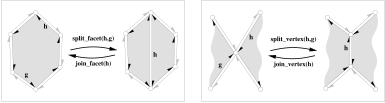
\includegraphics[width=\textwidth]{idraw/euler.ips}%
      }
    \end{center}
\end{ccTexOnly}

\begin{ccHtmlOnly}
    <CENTER>
    <img src="./euler_facet.gif" alt="Euler Operators: split/join_facet()"><P>
    </CENTER>
\end{ccHtmlOnly}


\ccMethod{Halfedge_handle split_facet( Halfedge_handle h,
                                       Halfedge_handle g);}
    {splits the facet incident to \ccc{h} and \ccc{g} into two facets
      with a new diagonal between the two vertices denoted by \ccc{h} and
      \ccc{g} respectively. The second (new) facet is a copy of the
      first facet. It returns the new diagonal. The time is
      proportional to the distance from \ccc{h} to \ccc{g} around the facet.
    \ccPrecond \ccc{h} and \ccc{g} are incident to the same facet.
               \ccc{h != g} (no loops). \ccc{h->next() != g} and
               \ccc{g->next() != h} (no multi-edges).}

\ccMethod{Halfedge_handle join_facet( Halfedge_handle h);}
    {joins the two facets incident to $h$. The facet incident to
      \ccc{h->opposite()} gets removed. Both facets might be
    holes. Returns the predecessor of $h$ around the facet. The invariant
    \ccc{join_facet( split_facet( h, g))} returns $h$ and keeps
    the polyhedron unchanged. The time is proportional to the size of the
    facet removed and the time to compute \ccc{h->prev()}.
    \ccPrecond \ccc{HDS} supports removal of halfedges and facets. The
    degree of both vertices incident to $h$ is at least three (no antennas).}

\begin{ccHtmlOnly}
    <CENTER>
    <img src="./euler_vertex.gif" alt="Euler Operator: split/join_vertex()"><P>
    </CENTER>
\end{ccHtmlOnly}

\ccMethod{Halfedge_handle split_vertex( Halfedge_handle h,
                                        Halfedge_handle g);}
    {splits the vertex incident to \ccc{h} and \ccc{g} into two vertices
      and connects them with a new edge. The second (new) vertex is a
      copy of the first vertex. It returns the new edge. The time is
      proportional to the distance from \ccc{h} to \ccc{g} around the vertex.
    \ccPrecond \ccc{h} and \ccc{g} are incident to the same vertex.
               \ccc{h != g} (no antennas).}

\ccMethod{Halfedge_handle join_vertex( Halfedge_handle h);}
    {joins the two vertices incident to $h$. The vertex denoted by
      \ccc{h->opposite()} gets removed. Returns the predecessor of
    $h$ around the vertex. The invariant 
    \ccc{join_vertex( split_vertex( h, g))} returns
    $h$ and keeps the polyhedron unchanged. 
    The time is proportional to the degree of the vertex removed and 
    the time to compute \ccc{h->prev()}.
    \ccPrecond \ccc{HDS} supports removal of vertices and halfedges. The
    size of both facets incident to $h$ is at least four (no multi-edges).}

% +-----------------------------------+
\newpage
\ccHeading{Euler Operators Modifying Genus}

\begin{ccTexOnly}
    \begin{center}
      \parbox{0.636\textwidth}{%
          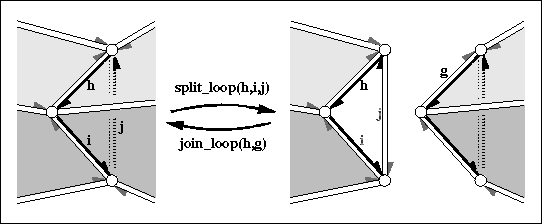
\includegraphics[width=0.636\textwidth]{idraw/euler_loop.ips}%
      }
    \end{center}
\end{ccTexOnly}

\begin{ccHtmlOnly}
    <CENTER>
    <img src="./euler_loop.gif" alt="Euler Operator: split/join_loop()"><P>
    </CENTER>
\end{ccHtmlOnly}

\ccMethod{Halfedge_handle split_loop( Halfedge_handle h,
                                      Halfedge_handle i,
                                      Halfedge_handle j);}
   {cuts the polyhedron into two parts along the cycle $(h,i,j)$.
    Three new vertices (one copy for each vertex in the cycle) and
    three new halfedges (one copy for each halfedge in the cycle), and
    two new triangles will be 
    created. $h,i,j$ will be incident to the first new triangle.
    The return value will be a halfedge iterator denoting the
    new halfedge of the second new triangle which was \ccc{h->opposite()}
    beforehand.
    \ccPrecond $h,i,j$ are distinct, consecutive halfedges of the
    polyhedron and form a cycle: i.e. \ccc{h->vertex() ==
    i->opposite()->vertex()}, \ldots, \ccc{j->vertex() ==
    h->opposite()->vertex()}. The six facets incident to $h,i,j$ are all
    distinct.
}

\ccMethod{Halfedge_handle join_loop( Halfedge_handle h,
                                     Halfedge_handle g);}
   {glues the boundary of two facets together.
    Both facets and the vertices of the facet loop $g$ gets removed. 
    Returns $h$.  Both facets might be holes.  
    The invariant \ccc{join_loop( h, split_loop( h, i, j))} 
    returns  $h$ and keeps the polyhedron unchanged.
    \ccPrecond \ccc{HDS} supports removal of vertices, halfedges, and 
    facets. The facets denoted by $h$ and $g$ are different and have an
    equal degree (i.e.~number of edges) $\geq 3$.} 

% +-----------------------------------+
\ccHeading{Modifying Facets and Holes}

\ccMethod{Halfedge_handle make_hole( Halfedge_handle h);}
    {removes the incident facet of $h$ and changes all halfedges incident 
    to the facet into border edges. Returns $h$. 
    See \ccc{erase_facet(h)} for a more generalized variant.    
    \ccPrecond \ccc{HDS} supports removal of facets. None of the 
    incident halfedges of the facet is a border edge.}

\ccMethod{Halfedge_handle fill_hole( Halfedge_handle h);}{
    fills a hole with a newly created facet. Makes all border halfedges
    of the hole denoted by $h$ incident to the new facet. Returns $h$.
  \ccPrecond \ccc{h.is_border()}.}

\begin{ccTexOnly}
    \begin{center}
      \parbox{\textwidth}{%
          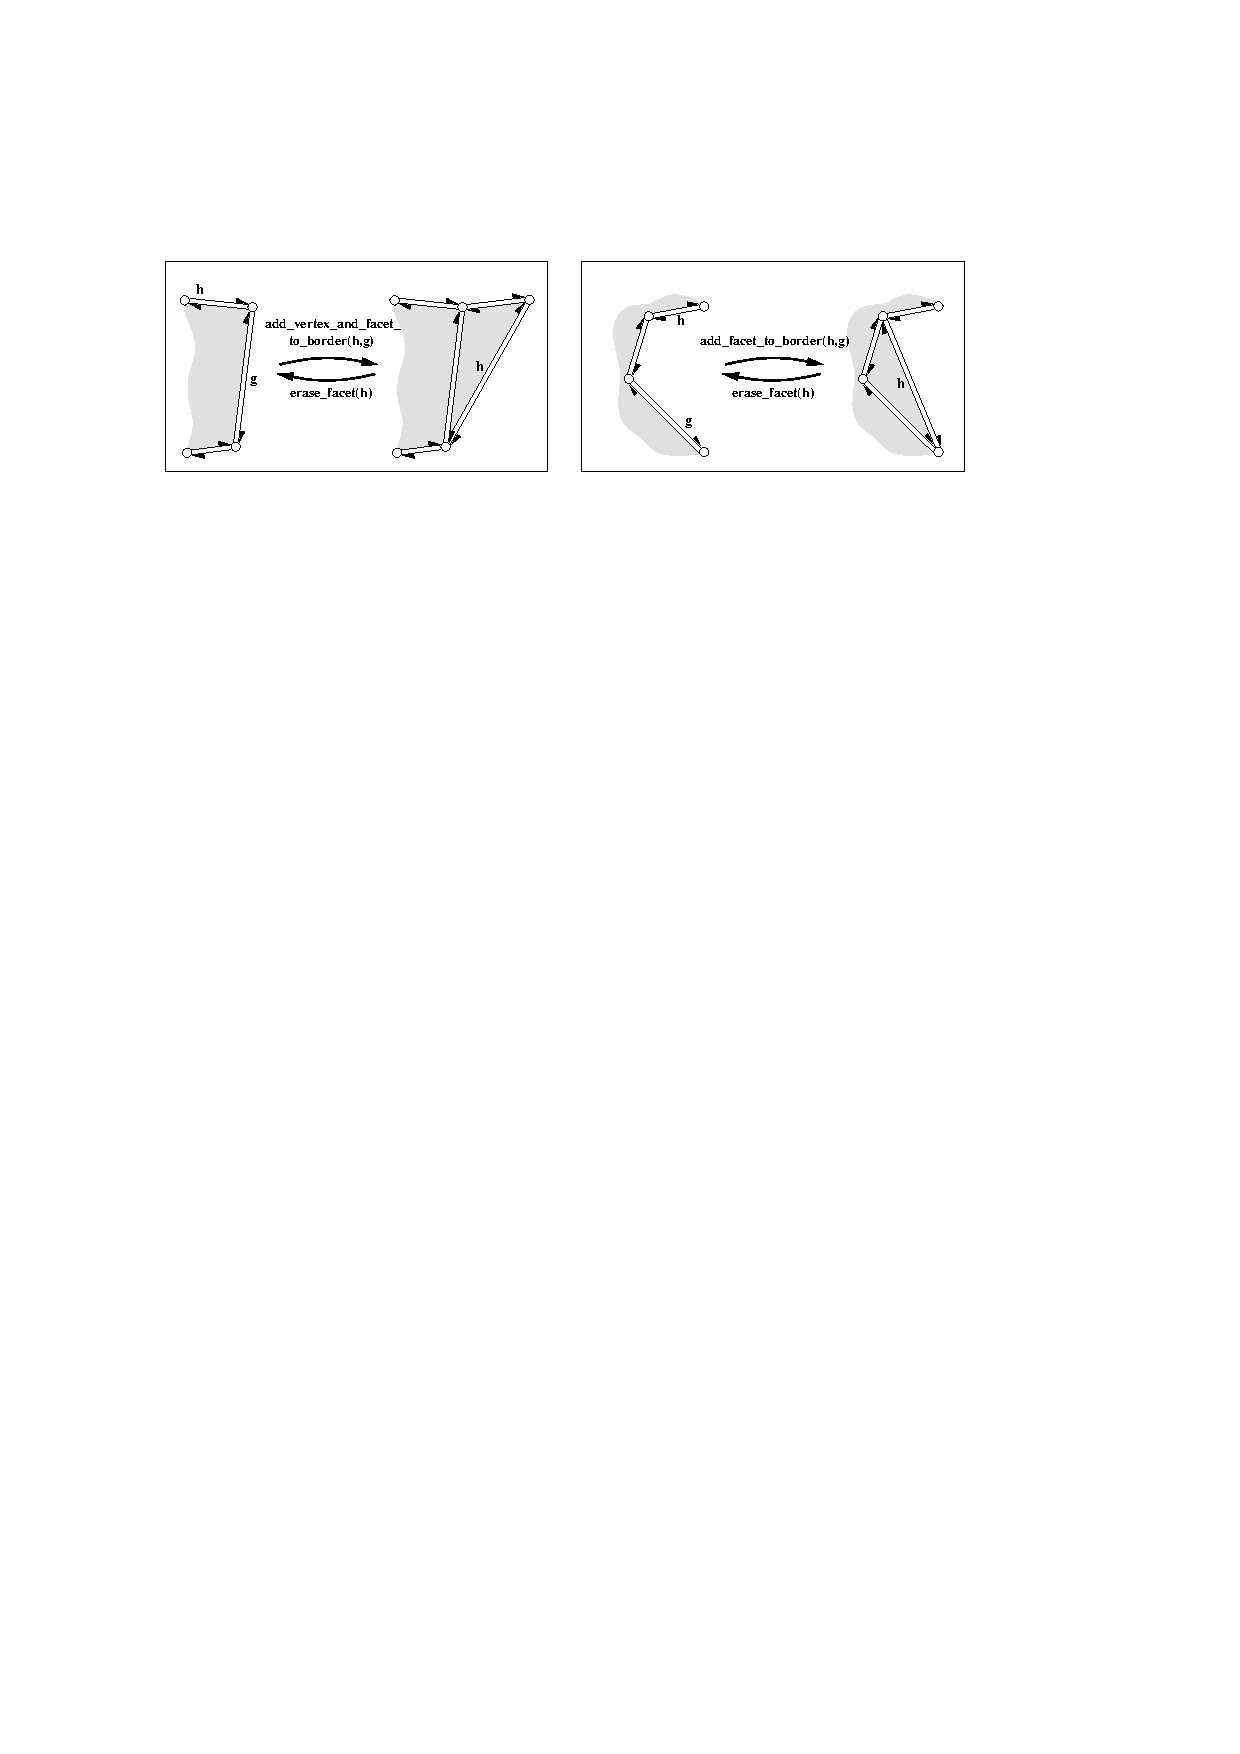
\includegraphics[width=\textwidth]{idraw/add_facet.ips}%
      }
    \end{center}
\end{ccTexOnly}

\begin{ccHtmlOnly}
    <CENTER>
    <img src="./add_facet1.gif" 
     alt="Modifying Facets and Holes: add_vertex_and_facet_to_border()"><P>
    </CENTER>
\end{ccHtmlOnly}


\ccMethod{Halfedge_handle add_vertex_and_facet_to_border( 
        Halfedge_handle h, Halfedge_handle g);}
   {creates a new facet within the hole incident to $h$
   and $g$ by connecting the tip of $g$ with the tip of $h$ 
   with two new halfedges and a new vertex and filling this separated
   part of the hole with a new facet, such that the new facet is
   incident to $g$. Returns the halfedge of the new edge that is
   incident to the new facet and the new vertex.
    \ccPrecond \ccc{h->is_border()}, \ccc{g->is_border()}, \ccc{h != g}, 
    and $g$ can be reached along the same hole starting with $h$.}

\begin{ccHtmlOnly}
    <CENTER>
    <img src="./add_facet2.gif" 
     alt="Modifying Facets and Holes: add_facet_to_border()"><P>
    </CENTER>
\end{ccHtmlOnly}

\ccMethod{Halfedge_handle add_facet_to_border( Halfedge_handle h,
                                               Halfedge_handle g);}
   {creates a new facet within the hole incident to $h$
   and $g$ by connecting the tip of $g$ with the tip of $h$ 
   with a new halfedge and filling this separated part
   of the hole with a new facet, such that the new
   facet is incident to $g$. Returns the halfedge of the new edge that
   is incident to the new facet.
   \ccPrecond \ccc{h->is_border()}, \ccc{g->is_border()}, \ccc{h != g}, 
   \ccc{h->next() != g}, and $g$ can be reached along the same hole
   starting with $h$.}


% +-----------------------------------+
\ccHeading{Erasing}

\ccMethod{void erase_facet( Halfedge_handle h);}
    {removes the incident facet of $h$ and changes all halfedges incident 
     to the facet into border edges or removes them from the
     polyhedral surface if they were already border edges.
     See \ccc{make_hole(h)} for a more specialized variant.    
     \ccPrecond \ccc{HDS} supports removal.}

\ccMethod{void erase_connected_component( Halfedge_handle h);}
    {removes the  vertices, halfedges, and facets that belong to the 
     connected component of $h$. \ccPrecond \ccc{HDS} supports removal.}

\ccMethod{void erase_all();}
    {removes all vertices, halfedges, and facets.}


% +-----------------------------------+
\ccHeading{Operations with Border Halfedges}

\begin{ccAdvanced}
  
Halfedges incident to an hole are called {\em border halfedges}. An
edge is a {\em border edge\/} if one of its two halfedges is a border
halfedges. The only requirement to work with border halfedges is
that the \ccc{Halfedge} class provides a member function
\ccc{is_border()} returning a \ccc{bool}. Usually, the halfedge data
structure supports facets and a \ccc{NULL} facet pointer will
indicate a border halfedge, but this is not the only possibility.
The \ccc{is_border()} predicate divides the edges into two classes,
the border edges and the non-border edges. The following
normalization reorganizes the sequential storage of the edges such
that the non-border edges precedes the border edges, and that for
each border edge the latter one of the two halfedges is a border
halfedge (the first one is a non-border halfedge in conformance with
the polyhedral surface definition). The normalization stores the
number of border halfedges and the halfedge iterator the border
edges start at within the data structure.  Halfedge insertion or
removal and changing the border status of a halfedge may invalidate
these values, which are not automatically updated.

\ccThree{Halfe}{dge_handleP.split_f}{}

\ccMethod{void   normalize_border();}
    {sorts halfedges such that the non-border edges precedes the
     border edges. For each border edge the halfedge iterator will
    reference the halfedge incident to the facet right before the
    halfedge incident to the hole.} 

\ccMethod{Size size_of_border_halfedges() const;}
    {number of border halfedges.
    \ccPrecond \ccc{normalize_border()} has been called and no
    halfedge insertion or removal and no change in border
    status of the halfedges have occurred since then.}

\ccMethod{Size size_of_border_edges() const;}
    {number of border edges. Since each border edge of a polyhedral
    surface has exactly one border halfedge,
    this number is equal to \ccc{size_of_border_halfedges()}.
    \ccPrecond \ccc{normalize_border()} has been called and no
    halfedge insertion or removal and no change in border
    status of the halfedges have occurred since then.}

\ccMethod{Halfedge_iterator  border_halfedges_begin();}
    {halfedge iterator starting with the border edges. The range
      [\ccStyle{halfedges_begin(), border_halfedges_begin()}) denotes
    all non-border edges. The range
    [\ccStyle{border_halfedges_begin(), halfedges_end()}) denotes all
    border edges.
    \ccPrecond \ccc{normalize_border()} has been called and no
    halfedge insertion or removal and no change in border
    status of the halfedges have occurred since then.}

\end{ccAdvanced}

% +-----------------------------------+
\ccHeading{Miscellaneous}

\ccMethod{void   inside_out();}
    {reverses facet orientation (incl.\ normal or plane equations).}

\begin{ccAdvanced}
\ccMethod{void  delegate( Modifier_base<HDS>& m);}
    {calls the \ccc{operator()} of the modifier $m$. See
    \ccc{Modifier_base} in the Support Library Manual for a
    description of modifier design and its usage.
    \ccPrecond The polyhedral surface must be valid when the modifier
    returns from execution.}
\end{ccAdvanced}

\ccMethod{bool is_valid( bool verbose = false, int level = 0) const;}
   {returns \ccc{true} if the polyhedral surface is combinatorially 
    consistent. If \ccc{verbose} is \ccc{true}, statistics are
    printed to \ccc{std::cerr}. For \ccc{level == 1} the normalization of the
    border edges is checked too. This method checks in particular level 3 of
    \ccc{Halfedge_data_structure_decorator::is_valid} from
    Section~\ref{sectionHdsDecorator} and that each facet is at least
    a triangle and that the two incident facets of a non-border edge are
    distinct.}

\ccMethod{bool normalized_border_is_valid( const HDS& hds, 
  bool verbose = false) const;}{%
    returns \ccc{true} if the border halfedges are in normalized 
    representation, which is when enumerating all halfedges with the
    iterator: The non-border edges precedes the border edges and for
    border edges, the second halfedge is the border halfedge. The halfedge
    iterator \ccc{border_halfedges_begin()} denotes the first border
    edge. If \ccc{verbose} is \ccc{true}, statistics are
    printed to \ccc{std::cerr}.
}

% +-----------------------------------+
\begin{ccAdvanced}
\ccHeading{Types for Tagging Optional Features}

\ccTwo{Polyhedron_3<Traits,HDS>:: Halfedge_vertex_circulator}{}

The following types are equal to either \ccStyle{Tag_true} or
\ccStyle{Tag_false}, depending on whether the named feature is
supported or not.

\ccNestedType{Supports_vertex_halfedge}{\ccc{Vertex::halfedge()}.}
\ccGlue
\ccNestedType{Supports_vertex_point}{\ccc{Vertex::point()}.}
\ccGlue
\ccNestedType{Supports_halfedge_prev}{\ccc{Halfedge::prev()}.}
\ccGlue
\ccNestedType{Supports_halfedge_vertex}{\ccc{Halfedge::vertex()}.}
\ccGlue
\ccNestedType{Supports_halfedge_facet}{\ccc{Halfedge::facet()}.}
\ccGlue
\ccNestedType{Supports_facet_halfedge}{\ccc{Facet::halfedge()}.}
\ccGlue
\ccNestedType{Supports_facet_plane}{\ccc{Facet::plane()}.}
\ccGlue
\ccNestedType{Supports_facet_normal}{\ccc{Facet::normal()}.}
\ccGlue
\ccNestedType{Supports_removal}{supports the
  removal of individual elements of a surface.}

\end{ccAdvanced}

\end{ccClassTemplate} 

% +========================================================================+

\begin{ccTexOnly}
    \begin{figure}
        \begin{center}
          \parbox{\textwidth}{%
              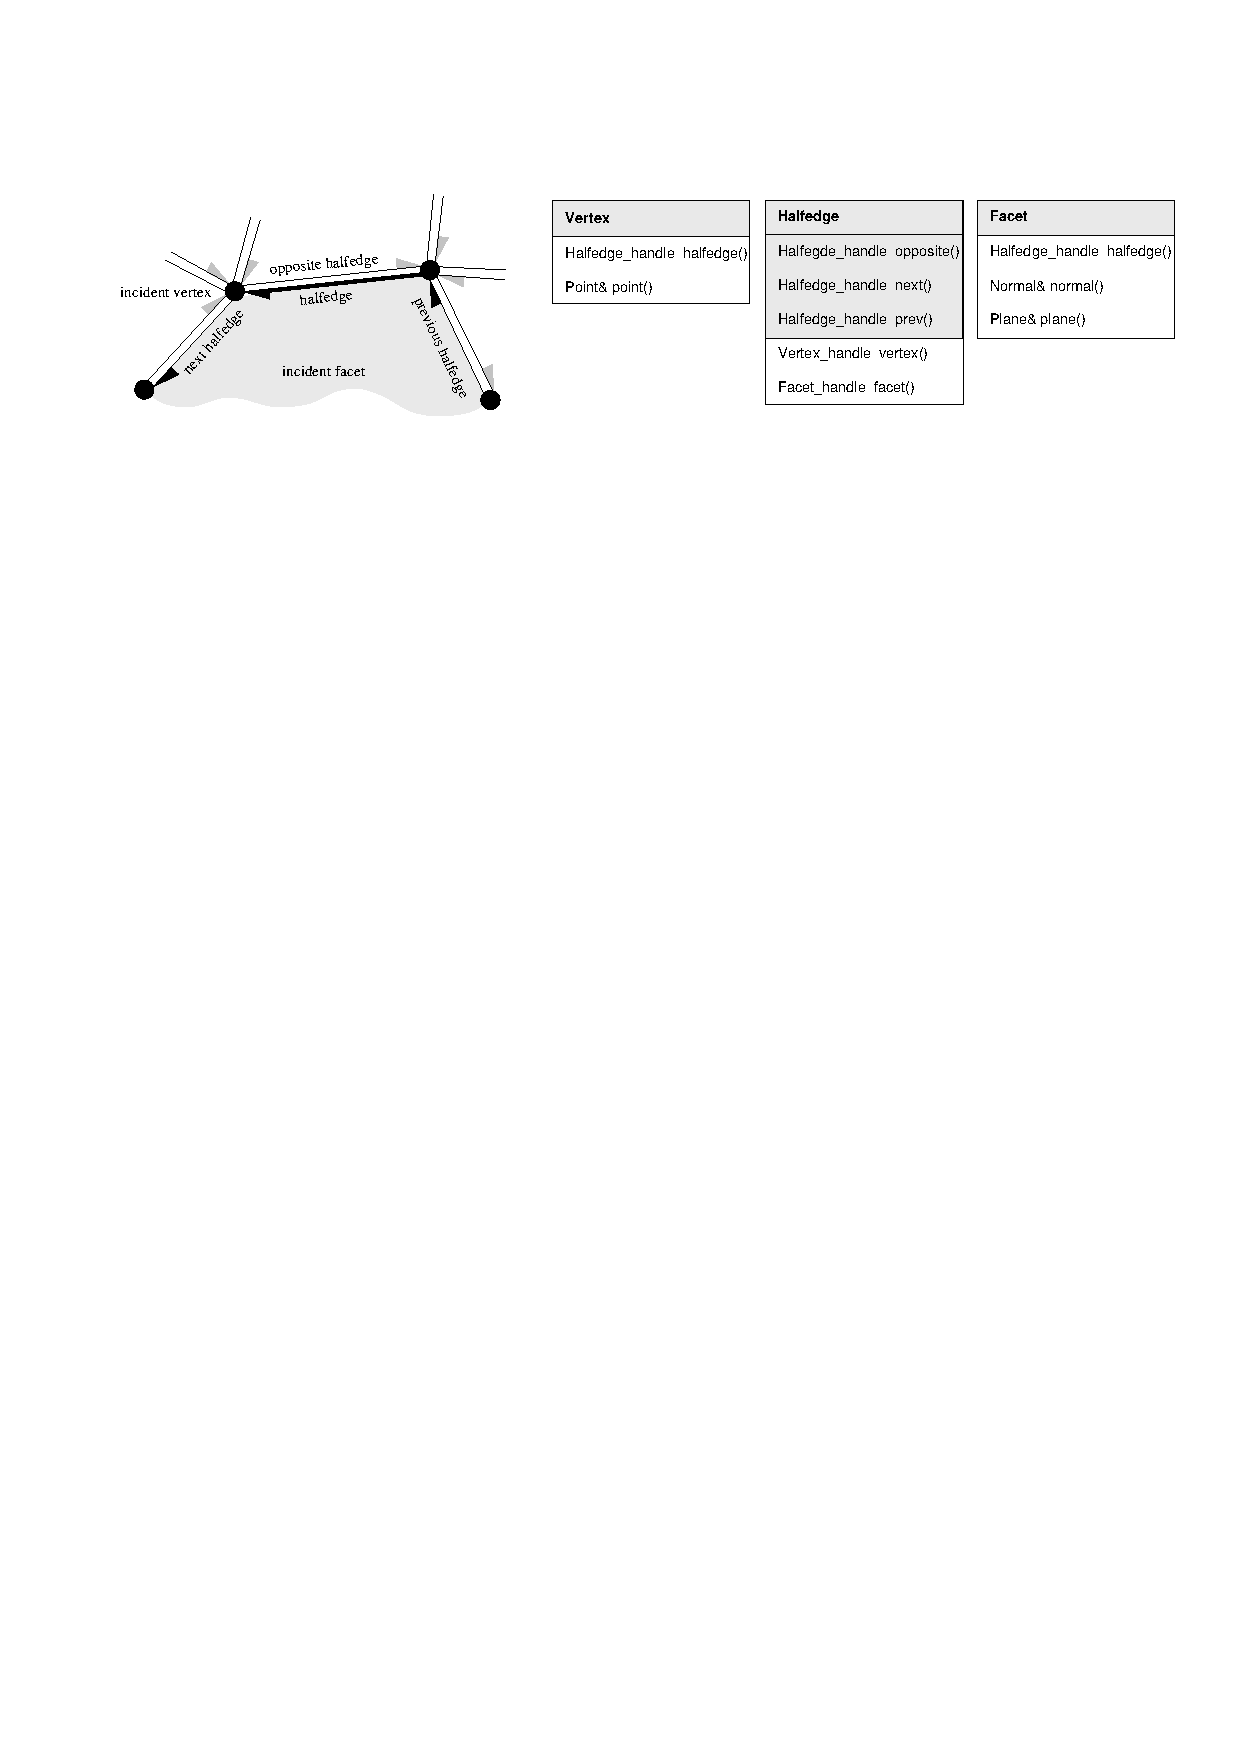
\includegraphics[width=\textwidth]{idraw/poly_optional.ips}%
          }
        \end{center}
        \caption{The three classes \protect\ccc{Vertex}, 
          \protect\ccc{Halfedge}, and 
          \protect\ccc{Facet} of the polyhedral surface. Member
          functions with shaded background are mandatory. The others
          are optionally supported.}
        \label{figurePolyOptionalMethods}
    \end{figure}
\end{ccTexOnly}

\begin{ccHtmlOnly}
    <CENTER>
    <A NAME="figurePolyOptionalMethods">
    <A HREF="./poly_optional.gif">
        <img src="./poly_optional_small.gif" 
             alt="Class Diagram"></A><BR>
    <A HREF="./poly_optional.gif">Figure:</A>
    The three classes <I>Vertex</I>, <I>Halfedge</I>, and 
          <I>Facet</I> of the polyhedral surface. Member
          functions with shaded background are mandatory. The others
          are optionally supported.
    </CENTER>
\end{ccHtmlOnly}


% +-------------------------------------------------------------+
\begin{ccClass}{Polyhedron_Vertex}
\subsection{Vertex of a Polyhedral Surface}

% +-----------------------------------+
\ccDefinition

A vertex optionally stores a point and a reference to an incident
halfedge that points to the vertex.  Type tags  as defined in
\ccc{Polyhedron_3} indicate whether these
member functions are supported.  
Figure~\ccTexHtml{\ref{figurePolyOptionalMethods}}{}\begin{ccHtmlOnly}
  <A HREF="Chapter_polyhedron.html#figurePolyOptionalMethods"><IMG 
  SRC="cc_ref_up_arrow.gif" ALT="reference arrow" WIDTH="10" HEIGHT="10"></A>
\end{ccHtmlOnly}
depicts the relationship between a halfedge and its incident halfedges,
vertices, and facets.

\ccCreationVariable{v}

% +-----------------------------------+
\ccTypes
\ccThree{Halfedge_handle}{h.next_on_vertex();;}{}
\ccThreeToTwo

\ccc{Vertex} defines the same types as \ccc{Polyhedron_3} except
the traits class.

% +-----------------------------------+
\ccHeading{Access Functions}

\ccMethod{Halfedge_handle halfedge();}{
    an incident halfedge pointing to \ccVar.}
\ccGlue
\ccMethod{Point&    point();}{the point.}

\ccMethod{Halfedge_around_vertex_circulator vertex_begin();}
    {circulator of halfedges around the vertex (clockwise).}

\end{ccClass}



% +-------------------------------------------------------------+
\begin{ccClass}{Polyhedron_Halfedge}
\subsection{Halfedge of a Polyhedral Surface}

% +-----------------------------------+
\ccDefinition

Figure~\ccTexHtml{\ref{figurePolyOptionalMethods}}{}\begin{ccHtmlOnly}
  <A HREF="Chapter_polyhedron.html#figurePolyOptionalMethods"><IMG 
  SRC="cc_ref_up_arrow.gif" ALT="reference arrow" WIDTH="10" HEIGHT="10"></A>
\end{ccHtmlOnly}
depicts the relationship between a
halfedge and its incident halfedges, vertices, and facets.  A halfedge
is an oriented edge between two vertices. It is always paired with its
counterpart that has the opposite direction. They are mutually linked
with the \ccc{opposite()} member function. If a halfedge is incident
to a facet the \ccc{next()} member function points to the successor
halfedge around this facet. For border edges the \ccc{next()} member
function points to the successor halfedge along some hole (which might
not be uniquely determined in situations with more than one hole at a
vertex).  An invariant is that successive assignments of the form
\ccc{h = h->next()} cycles counterclockwise around the facet and
traverses all halfedges incident to this facet. A similar invariant is
that successive assignments of the form \ccc{h =
  h->next()->opposite()} cycles clockwise around the vertex and
traverses all halfedges incident to this vertex. Two circulators are
provided for these circular orders. \ccc{next()} and \ccc{opposite()}
are mandatory functions for each instantiation of polyhedral surfaces.
The other member functions are optional
as indicated with the type tags defined in
\ccc{Polyhedron_3}, see Section~\ref{sectionPolyhedron}.
The \ccc{prev()} member function points to the preceding halfedge around
the same facet.  Handles to the incident vertex and facet are
optionally stored.

\ccCreationVariable{h}
\ccThree{Halfedge_handle}{h.next_on_vertex();;}{}

% +-----------------------------------+
\ccTypes

\ccc{Halfedge} defines the same types as \ccc{Polyhedron_3} except
the traits class.

% +-----------------------------------+
\ccHeading{Access Functions}

\ccMethod{Halfedge_handle opposite();}{the opposite halfedge.}
\ccGlue
\ccMethod{Halfedge_handle next();}{the next halfedge around the facet.}
\ccGlue
\ccMethod{Halfedge_handle prev();}{the previous halfedge around the facet.}
\ccGlue
\ccMethod{Vertex_handle   vertex();}{the incident vertex.}
\ccGlue
\ccMethod{Facet_handle    facet();}{the incident facet. If \ccVar\
          is a border halfedge the result is a singular value for the
          handle.}
\ccGlue
\ccMethod{Halfedge_handle next_on_vertex() const;}{
    the next halfedge around the vertex (clockwise). Is equal
    to \ccc{h.next()->opposite()}.}
\ccGlue
\ccMethod{Halfedge_handle prev_on_vertex() const;}{
    the previous halfedge around the vertex (counterclockwise). 
    Is equal to \ccc{h.opposite()->prev()}.}

\ccMethod{Halfedge_around_vertex_circulator vertex_begin();}
    {circulator of halfedges around the vertex (clockwise).}

\ccMethod{Halfedge_around_facet_circulator facet_begin();}
    {circulator of halfedges around the facet (counterclockwise).}

\ccMethod{bool             is_border() const;}
    {is true if \ccVar\ is a border halfedge.}
\ccGlue
\ccMethod{bool             is_border_edge() const;}
    {is true if \ccVar\ or \ccc{h.opposite()} is a border halfedge.}

% +-----------------------------------+
\ccImplementation

The methods \ccc{prev()} and \ccc{prev_on_vertex()} work in constant
time if \ccc{Supports_halfedge_prev} $\equiv$
\ccc{Tag_true}. Otherwise both methods search for the previous
halfedge around the incident facet.

\end{ccClass}


% +-------------------------------------------------------------+
\begin{ccClass}{Polyhedron_Facet}
\subsection{Facet of a Polyhedral Surface}

% +-----------------------------------+
\ccDefinition

A facet optionally stores a normal vector, a plane, and a reference to
an incident halfedge that points to the facet.  If a plane is
supported the normal is taken from the plane equation.  The type tags
as defined in \ccc{Polyhedron_3} indicates whether these
member functions are supported, see Section~\ref{sectionPolyhedron}.
Figure~\ccTexHtml{\ref{figurePolyOptionalMethods}}{}\begin{ccHtmlOnly}
  <A HREF="Chapter_polyhedron.html#figurePolyOptionalMethods"><IMG 
  SRC="cc_ref_up_arrow.gif" ALT="reference arrow" WIDTH="10" HEIGHT="10"></A>
\end{ccHtmlOnly}
depicts the relationship between a
halfedge and its incident halfedges, vertices, and facets.

\ccCreationVariable{f}

% +-----------------------------------+
\ccTypes

\ccc{Facet} defines the same types as \ccc{Polyhedron_3} except
the traits class.

% +-----------------------------------+
\ccHeading{Access Functions}

\ccMethod{Halfedge_handle halfedge() const;}{
    an incident halfedge pointing to \ccVar.}
\ccGlue
\ccMethod{Normal&   normal();}{the normal vector. If a plane equation
    is supported, only a value of the normal vector is returned 
    (no reference).}
\ccGlue
\ccMethod{Plane&    plane();}{the supporting plane of the facet.}

\ccMethod{Halfedge_around_facet_circulator facet_begin();}
    {circulator of halfedges around the facet (counterclockwise).}

\end{ccClass}


% +========================================================================+
\newpage
\ccHtmlNoClassToc
\begin{ccClass}{Polyhedron_traits}
\section{Requirements for a \protect\ccc{Polyhedron_traits}}
% +========================================================================+
\label{sectionPolyTraits}
\ccCreationVariable{traits}

\ccDefinition  

A model for the \ccClassName\ concept must provide the following
types, operations and restrictions with respect to the halfedge data
structure \ccc{HDS} used in the polyhedral surface.

\ccTypes

\ccNestedType{Point}{point type equal to
  \ccc{HDS::Point}, if points are supported.}
\ccGlue
\ccNestedType{Normal}{normal vector equal to
  \ccc{HDS::Facet::Normal}, if normals are supported.}
\ccGlue
\ccNestedType{Plane}{plane equation equal to
  \ccc{HDS::Facet::Plane}, if plane equations are
  supported.}

\ccOperations

\ccTagFullDeclarations

\ccMethod{void reverse_normal( Normal& n) const;}{
    reverses the orientation of the normal vector \ccc{n}. Only needed
    if normal vectors are supported.}

\ccMethod{void reverse_plane( Plane& p) const;}{
    reverses the orientation of the plane equation \ccc{p}. Only
    needed if plane equations are supported.}

\ccTagDefaults

\ccSeeAlso

\ccc{Polyhedron_3} and \ccc{Polyhedron_default_traits_3}.

\end{ccClass}

% +========================================================================+
\ccHtmlNoClassToc
\begin{ccClassTemplate}{Polyhedron_default_traits_3<R>}
\section{Models of \protect\ccc{Polyhedron_traits}}
% +========================================================================+
\label{sectionPolyTraitsModels}
\ccCreationVariable{traits}

\ccDefinition

\ccClassTemplateName\ is a model of the \ccc{Polyhedron_traits} concept
from Section~\ref{sectionPolyTraits} based on the \cgal-kernel. It
defines \ccc{Point_3<R>} as points, \ccc{Vector_3<R>} as
surface normal vectors, and \ccc{Plane_3<R>} as plane equations.

\ccInclude{CGAL/Polyhedron_default_traits_3.h}

\end{ccClassTemplate}




% +========================================================================+
%%\section[Additional Requirements and a Default Model for a
%%         \protect\ccc{Halfedge_data_structure}]{Additional Requirements
%%           and a Default Model\\ for a \protect\ccc{Halfedge_data_structure}}
\section{Additional Requirements and a Default Model for a
          \protect\ccc{Halfedge_data_structure}}
% +========================================================================+
\label{sectionPolyHds}

The additional requirements allow to work with normal vectors or plane
equations associated to facets as flexible as with the point type
associated to vertices. The storage of either a normal vector or a
plane equation in a facet is optional.

% +-------------------------------------------------------------+
\subsection{Additional Requirements}

\ccThree{Halfedge_iterator}{hds.capacity_of_halfedges() const;;}{}
\ccThreeToTwo

\ccDefinition

A halfedge data structure used for polyhedral surfaces must be a model
of the \ccc{Halfedge_data_structure} concept as described in
Section~\ref{sectionHds} and additionally provides the following types
and operations for the local \ccc{Facet} type to support optionally
surface normals or plane equations for facets.

\ccHtmlNoClassFile
\ccHtmlNoClassLinks
\ccHtmlNoClassIndex
\begin{ccClass}{Facet}
\ccCreationVariable{f}

% +-----------------------------------+
\ccTypes

Types for (optionally) associated geometry in facets. If they
are not supported the respective types are \ccc{void*}.

\ccNestedType{Normal}{surface normal vector stored in facets.}
\ccGlue
\ccNestedType{Plane}{plane equation stored in facets.}

% +-----------------------------------+
\ccOperations

The member functions for the normal vector or the plane equation are
only needed if the respective feature is supported. If plane equations
are supported, a member function for the normal vector is necessary,
though only with a value semantic of the return value (no reference as
return value).

\ccTagFullDeclarations

\ccMethod{Normal&       normal();}{the surface normal vector.}
\ccGlue
\ccMethod{const Normal& normal() const;}{}

\ccMethod{Plane&       plane();}{the plane equation.}
\ccGlue
\ccMethod{const Plane& plane() const;}{}

\ccTagDefaults

% +-----------------------------------+
\ccHeading{Types for Tagging Optional Features}

The nested types below are either equal to \ccStyle{Tag_true} or
\ccStyle{Tag_false}, depending on whether the named member function
is supported or not.

\ccHtmlNoLinks
\ccNestedType{Supports_facet_normal}{\ccc{normal()}.}
\ccGlue
\ccHtmlNoLinks
\ccNestedType{Supports_facet_plane}{\ccc{plane()}.}

The following dependencies among these options and those of the
\ccc{Halfedge} type must be regarded:

\ccc{Supports_facet_normal} $\equiv$ \ccc{Tag_true} $\Longrightarrow$
\ccc{Supports_halfedge_facet} $\equiv$ \ccc{Tag_true}.
\\
\ccc{Supports_facet_plane} $\equiv$ \ccc{Tag_true} $\Longrightarrow$
\ccc{Supports_halfedge_facet} $\equiv$ \ccc{Tag_true}.

\end{ccClass}

% +-------------------------------------------------------------+
\begin{ccClassTemplate}{Halfedge_data_structure_polyhedron_default_3<R>}
\subsection{The Default Halfedge Data Structure for Polyhedra}
\label{sectionPolyHdsDefault}

\ccCreationVariable{hds}

\ccDefinition

The default \ccClassTemplateName\ implements all incidences supported
by the \ccc{Halfedge_data_structure} concept. It chooses geometry
types from the \cgal-kernel as determined with the representation
class \ccc{R}. It stores a point of type \ccc{Point_3<R>} in each
vertex and a plane equation of type \ccc{Plane_3<R>} in each facet.

\ccInclude{CGAL/Halfedge_data_structure_polyhedron_default_3.h}

\ccImplementation

The default halfedge data structure provided for polyhedra is a wrapper for
the class \ccc{Halfedge_data_structure_using_list} using the
\ccc{Vertex_max_base<Point_3<R>>},
\ccc{Halfedge_max_base} and \ccc{Polyhedron_facet_base_3}
models, see Section~\ref{sectionHdsUsingList} to
\ref{sectionHdsBasesModels} and \ref{sectionPolyHdsBases}.

\end{ccClassTemplate}

% +-------------------------------------------------------------+
\subsection{Models of \protect\ccc{Facet_base}}
\label{sectionPolyHdsBases}

\cgal\ currently provides a model for the \ccc{Facet_base} concept
specifically tailored for polyhedral surfaces. Other models can be found
in Section~\ref{sectionHdsBasesModels}.

\ccTwo{class Polyhedron_facet_base_3 ();;}{}

\ccStruct{template <class R> class Polyhedron_facet_base_3 {};}
    {defines the maximal facet functionality for polyhedra including
     halfedge pointer and a plane equation of type \ccc{Plane_3<R>}.}

\ccSeeAlso

\ccc{Vertex_min_base}, \ldots, \ccc{Facet_max_base}, and\\
\ccc{Halfedge_data_structure_polyhedron_default_3}.



% +========================================================================+
\newpage
\ccHtmlNoClassToc
\begin{ccClassTemplate}{Polyhedron_incremental_builder_3<HDS>}
\section{An Incremental Builder for Polyhedral Surfaces}
% +========================================================================+
\label{sectionPolyIncrBuilder}

\ccCreationVariable{B}

\ccDefinition  

\ccClassTemplateName\ is an auxiliary class that supports the
incremental construction of polyhedral surfaces. This is for example
convenient when constructing polyhedral surfaces from file formats
like the Object File Format (OFF)~\cite{p-gmgv15-94},
OpenInventor~\cite{w-impoo-94} or VRML~\cite{bpp-vrml-95,vrmls-96}.
\ccClassTemplateName\ needs access to the internal halfedge data
structure of type \ccc{HDS} of the polyhedral surface. It is intended
to be used within a modifier, see \ccc{Modifier_base} in the
Support Library Manual.

The incremental builder might be of broader interest for other
halfedge data structures as well, but it is specifically bound to the
definition of polyhedral surfaces given here. During construction all
conditions of polyhedral surfaces are checked and in case of violation
an error status is set. A diagnostic message will be printed to
\ccc{std::cerr} if the \ccc{verbose} flag has been set at construction time.

The incremental construction starts with a list of all point
coordinates and concludes with a list of all facet polygons. Edges are
not explicitly specified. They are derived from the vertex incidence
information provided from the facet polygons. The polygons are given as a
sequence of vertex indices.  The halfedge data structure \ccc{HDS} must
support vertices (i.e.~\ccc{Supports_halfedge_vertex} $\equiv$
\ccc{Tag_true}). The correct protocol of method calls to build a
polyhedral surface is given as a regular expression below. Vertices and
facets can be added in arbitrary order as long as
\ccc{add_vertex_to_facet()} refers only to vertex indices that are
already known.

{\it
    \hspace*{6mm} begin\_surface $($add\_vertex $|$ 
                  $($begin\_facet add\_vertex\_to\_facet$\:*$
                            end\_facet\/$))\:*$ end\_surface
}

\ccTypes
\ccTwo{Polyhedron_incremental_builder_3<HDS>:: Point}{}

\ccNestedType{Halfedge_data_structure}{halfedge data structure \ccc{HDS}.}
\ccGlue
\ccNestedType{Point}{its point type.}
\ccGlue
\ccNestedType{Size}{its size type.}

\ccCreation
\ccThree{void}{B.remove_unconnected_vertices();}{}
\ccThreeToTwo

\ccConstructor{Polyhedron_incremental_builder_3(HDS& hds, 
               bool verbose = false);}
 {stores a reference to the halfedge data structure \ccc{hds} of a
   polyhedral surface in its internal state. An existing polyhedral
   surface in \ccc{hds} remains unchanged. The incremental builder
   appends the new polyhedral surface. If \ccc{verbose} is \ccc{true},
   diagnostic messages will be printed to \ccc{std::cerr} in case of
   malformed input data.}

\newpage
\ccOperations

\ccMethod{void begin_surface( Size v, Size f, Size h = 0);}
{starts the construction. $v$ is the number of vertices
    to expect, $f$ the number of facets, and $h$ the number of
    halfedges. If $h$ is unspecified (\ccc{== 0}) it is estimated using
    Euler's equation (plus 5\% for the so far unknown holes and genus of
    the object). These values are used to reserve space in the
    halfedge data structure \ccc{hds}. If the representation supports
    insertion these values do not restrict the class of constructible
    polyhedra. If the representation does not support insertion the
    object must fit into the reserved sizes.}  

\ccMethod{void add_vertex( const Point& p);}{
    adds $p$ to the vertex list.}  
\ccGlue
\ccMethod{void begin_facet();}{starts a facet.}
\ccGlue
\ccMethod{void add_vertex_to_facet( Size i);}{adds a vertex with
  index $i$ to the current facet. The first point added with
  \ccc{add_vertex()} has the index 0.}
\ccGlue
\ccMethod{void end_facet();}{ends a facet.}
\ccGlue
\ccMethod{void end_surface();}{ends the construction.}

\ccMethod{bool error() const;}{returns error status of the builder.}
\ccGlue
\ccMethod{void rollback();}{undoes all changes made to the halfedge
  data structure since the last \ccc{begin_surface()}.}

\ccMethod{bool check_unconnected_vertices();}{returns
  \ccc{true} if unconnected vertices are detected. If \ccc{verbose} was set to
  \ccc{true} (see the constructor above) debug information about the
  unconnected vertices is printed.}

\ccMethod{bool remove_unconnected_vertices();}{returns
  \ccc{true} if all unconnected vertices could be removed successfully.
  This happens either if no unconnected vertices had appeared or if the
  halfedge data structure supports the removal of individual elements.}

\end{ccClassTemplate}


% +========================================================================+
\newpage
\section{Examples Using Polyhedral Surfaces}
% +========================================================================+
\label{sectionPolyExamples}

Examples of different halfedge data structures can be found in
Section~\ref{sectionHdsExamples}.


% +-------------------------------------------------------------+
\subsection{First Example Using Defaults}

The first example instantiates a polyhedron using the default traits
class, the default halfedge data structure, and creates a tetrahedron.

\ccIncludeVerbatim{examples/Polyhedron/polyhedron_prog_simple.C}

% +-------------------------------------------------------------+
\subsection{Example with Geometry in Vertices}

This example creates a tetrahedron initialized with four points. In
addition it demonstrates the use of the vertex iterator and the access
to the point in the vertices. The output of
the program will be {\tt (1 0 0) (0 1 0) (0 0 1) (0 0 0)}.

\ccIncludeVerbatim{examples/Polyhedron/polyhedron_prog_tetra.C}

% +-------------------------------------------------------------+
\subsection{Example Computing Plane Equations}

This example computes the plane equations for the facets of a tetrahedron.
The actual plane computation is provided in the user defined function
{\tt compute\_plane\_equations}. We assume
here strictly convex facets and exact arithmetic. In our example a
homogeneous representation with {\tt int} coordinates is sufficient.
The output of the program are the four plane equations.

\ccIncludeVerbatim{examples/Polyhedron/polyhedron_prog_normals.C}

% +-------------------------------------------------------------+
\subsection{Example Declaring a Point Iterator}

It might be preferable to have an iterator enumerating all points
directly instead of all vertices as in the previous example. Such an 
iterator could be used in other algorithms, for example a convex hull
computation. The following declaration gives us such a point iterator.

\begin{verbatim}
#include <CGAL/Iterator_project.h>
#include <CGAL/function_objects.h>

typedef Polyhedron::Vertex                                   Vertex;
typedef Polyhedron::Vertex_iterator                          Vertex_iterator;
typedef Polyhedron::Point                                    Point;
typedef Polyhedron::Difference                               Difference;
typedef Polyhedron::iterator_category                        iterator_category;
typedef Project_point<Vertex>                                Project_point;
typedef Iterator_project<Vertex_iterator, Project_point,
        Point&, Point*, Difference, iterator_category>       Point_iterator;
\end{verbatim}

The {\tt for}-loop of the previous example could now be replaced with
the following loop:

\begin{verbatim}
    Point_iterator begin = P.vertices_begin();
    for ( ; begin != P.vertices_end(); ++begin)
        cout << "(" << (*begin) << ") ";
\end{verbatim}



% +-------------------------------------------------------------+
\subsection{Example Writing Object File Format (OFF) with STL Algorithms}

The following example creates a tetrahedron and writes it to
\ccc{cout} using the Object File Format (OFF)~\cite{p-gmgv15-94}.
The example makes advanced use of \stl\ algorithms (\ccc{copy},
\ccc{distance}), \stl\ \ccc{ostream_iterator} and \cgal\ circulators.

\ccIncludeVerbatim{examples/Polyhedron/polyhedron_prog_off.C}


% +------------------------------------------------------------------------+
\subsection{Example Using the Incremental Builder and Modifier Mechanism}

The \ccc{Polyhedron_incremental_builder_3} class is used to create
a triangle using the modifier mechanism as described in the Support
Library Manual.

\ccIncludeVerbatim{examples/Polyhedron/polyhedron_prog_incr_builder.C}

% +--------------------------------------------------------+

% EOF
